\documentclass[10pt, english, xcolor={dvipsnames}]{beamer}
\mode<presentation> {
	\usetheme{Copenhagen}
	% \usetheme{Madrid}
%	\setbeamertemplate{itemize item}{\color{black}\normalsize\textbullet}
}

\usepackage{../macros}
\usepackage{style}
\usepackage{../katla-preamble}

\usepackage{contour}

% TODO: find a new font for math mode
% TODO: change theorem style


% \setbeamertemplate{title page}{
%     \begin{center}
%         \begin{beamercolorbox}[sep=8pt,center,shadow=true,rounded=true]{title}
%             \usebeamerfont{title}\inserttitle\par%
%           %  \vspace{0.5cm} % Espacement vertical ajouté
%         \end{beamercolorbox}%
%       %  \vspace{6.5cm} % Espacement vertical ajouté
%       %  \begin{beamercolorbox}[sep=8pt,center,shadow=true,rounded=true]{author}
% 	    %     \usebeamerfont{author}\color{white}\contour{black}{\insertauthor}\par%
% 	    % \end{beamercolorbox}%
% %	    \vspace{0.5cm} % Vertical space added
% 	    % \begin{beamercolorbox}[sep=8pt,center,shadow=true,rounded=true]{institute}
% 	    %     \usebeamerfont{institute}\color{white}\contour{black}{\insertinstitute}\par%
% 	    % \end{beamercolorbox}%
% %	    \vspace{0.5cm} % Vertical space added
% 	    % \begin{beamercolorbox}[sep=8pt,center,shadow=true,rounded=true]{date}
% 	    %     \usebeamerfont{date}\color{white}\contour{black}{\insertdate}\par%
% 	    % \end{beamercolorbox}%
%     \end{center}
% }

\title[Varieties of Semiring Solvers]{Varieties of Semiring Solvers via Multicategorical and Algebraic Constructions}

\author{MAZOYER Amaury}

\institute{ENS de Lyon}
%\institute{\contour{black}{\color{white}MPI}}

\date{May 4 -- July 31 2026}

\begin{document}

\fontsize{10pt}{14pt}\selectfont

\begin{frame}
\titlepage

\centering
supervised by Ohad Kammar of the University of Edinburgh, School of Informatics
\end{frame}

\begin{frame}[fragile, t]{Motivation}
  \begin{block}{Problem}
      Prove formally that $\forall a, b \in \R, (a + b)^2 = a^2 + 2ab + b^2$.
      % Prove formally that \texttt{(a + b) * (a + b) = a * a + 2 * a * b + b * b}.
  \end{block}

  \structure{Formal proof:} 10 axiom invocations.
\pause
\vspace{0.3cm}

\structure{Automation:}
\begin{minted}{coq}
Require Import Ring.
Goal forall a b : R, (a + b)^2 = a^2 + 2*a*b + b^2.
Proof. intro a b. ring. Qed.
\end{minted}
\pause
\begin{figure}
  \centering
\begin{tikzpicture}
  \node[draw, align=center] (node1) at (0.12,1.5) {monoid\\solver};
  \node[draw=none, node font=\scriptsize] at (0.12,2.17) {``multiplication''};
  \node[draw=none, node font=\scriptsize] at (5.87,2.39) {``addition''};
  \node[draw, align=center] (node3) at (5.87,1.5) {commutative\\monoid\\solver};
  \node[draw, shape=ellipse] (node2) at (2.78,1.5) {combining};


  \node[draw, align=center] (node4) at (2.78,0.01) {semiring\\solver};
  \draw[->] (node2.south) -- (node4.north);
  \draw[->] (node1.east) -- (node2.west);
  \draw[->] (node3.west) -- (node2.east);
\end{tikzpicture}
\end{figure}
\end{frame}

\begin{frame}[t]{State of the art}
  \structure{Original \textsc{Frex} framework}

  Free algebras / free extensions for equational reasoning\footnote<1->{\citetitle{frex_origin}, \citeauthor{frex_origin}, \citeyear{frex_origin}}
  \pause

  \medskip
  
  \structure{Subsequent work}
  
  Using \textsc{Frex} to build solvers, with an Idris 2 formalisation\footnote<2->{\citetitle{idris_frex}, \citeauthor{idris_frex}, \citeyear{idris_frex}}
  \pause
  \medskip
  
  \structure{Existing modular constructions}
  
  Modular frex construction for involutive algebras\footnote<3->{\citetitle{involutive_frex}, \citeauthor{involutive_frex}, \citeyear{involutive_frex}}
  \pause
  \medskip

  \structure{Gap before this work}

  No modular construction for distributive combinations
  \pause
  \medskip

  \structure{Other solvers}

  Rocq's reflexion-based semiring/ring solver, state of the art\footnote<5->{\citetitle{coq_ring}, \citeauthor{coq_ring}, \citeyear{coq_ring}}
\end{frame}


\begin{frame}{Practical payoff}
  \centering
  \hspace*{-0.6cm}
  \resizebox{1.1\textwidth}{!}{%
  \begin{tabular}{|l|l|l|>{\centering\arraybackslash}p{3.5cm}|>{\centering\arraybackslash}p{3.5cm}|>{\centering\arraybackslash}p{3.5cm}|}
  \hline
  \multicolumn{3}{|c|}{\textbf{Multiplicative structure}} &
  \multicolumn{3}{c|}{\textbf{Additive structure}} \\ \hline
  \textbf{Theory} & \textbf{Comm.} & \textbf{Inv.} &
  \makecell{\textbf{Comm. Semigroup}} &
  \makecell{\textbf{Comm. Monoid}} &
  \makecell{\textbf{Abelian Group}} \\ \hline

  \multirow{4}{*}{\small\textbf{Semigroup}}
  & \multirow{2}{*}{\textbf{Mere}} & \textbf{Mere} & $\P(\Sigma^+) \setminus \{\varnothing\}$ & $\P(\Sigma^+)$ & $\Z \la \Sigma^+ \ra$ \\ \cline{3-6}
  &                                   & \textbf{Inv.} & $\lp \P(\Sigma^+) \setminus \{\varnothing\}, -^R \rp$ & $\lp \P(\Sigma^+), -^R \rp$ & $\lp \Z \la \Sigma^+ \ra, \rev \rp$ \\ \cline{2-6}
  & \multirow{2}{*}{\textbf{Comm.}} & \textbf{Mere} & $2\N_{>0}$ & $2\N$ & $2\Z$ \\ \cline{3-6}
  &                                   & \textbf{Inv.} & $\mathfrak m_n^\sigma \setminus \{0\}$ & $\mathfrak m_n^\sigma$ & $\lp 2\Z[\ii], \overline{-} \rp$ \\ \hline

  \multirow{4}{*}{\textbf{Monoid}}
  & \multirow{2}{*}{\textbf{Mere}} & \textbf{Mere} & $\P(\Sigma^*) \setminus \{\varnothing\}$, $M_n(\N_{>0})$ & $\P(\Sigma^*)$ , $M_n(\N)$ & $M_n(\Z)$ \\ \cline{3-6}
  &                                   & \textbf{Inv.} & $\lp M_n(\N_{>0}), -^T\rp$, $\lp\P(\Sigma^*) \setminus \{\varnothing\}, -^R\rp$ & $\lp M_n(\N), -^T\rp$, $\lp \P(\Sigma^*), -^R\rp$, $\Rel(X)$ & $\lp M_n(\Z), -^T \rp$ \\ \cline{2-6}
  & \multirow{2}{*}{\textbf{Comm.}} & \textbf{Mere} & $\N_{>0}$ & $\color{red}\Circled[inner xsep=7pt, inner ysep=7pt]{\N}$ & $\color{red}\Circled[inner xsep=7pt, inner ysep=5pt]{\Z,\; \R,\; \C}$ \\ \cline{3-6}
  &                                   & \textbf{Inv.} & $\N_\sigma\brak{X_1, \dots, X_n} \setminus \{0\}$ & $\N_\sigma\brak{X_1, \dots, X_n}$ & $(\C, \overline{-})$, $\Z_\sigma\brak{X_1, \dots, X_n}$ \\ \hline

  \multirow{4}{*}{\textbf{Group}}
  & \multirow{2}{*}{\textbf{Mere}} & \textbf{Mere} & $T_{n,\Delta_{>0}}(\R)$ & \textbf{impossible} nontrivially & \textbf{impossible} nontrivially \\ \cline{3-6}
  &                                   & \textbf{Inv.} & $\bigl( T_{n,\Delta_{>0}}(\R), -^\dagger \bigr)$ & \textbf{impossible} nontrivially & \textbf{impossible} nontrivially \\ \cline{2-6}
  & \multirow{2}{*}{\textbf{Comm.}} & \textbf{Mere} & $\R_{>0}$ & \textbf{impossible} nontrivially & \textbf{impossible} nontrivially \\ \cline{3-6}
  &                                   & \textbf{Inv.} & $(\C_{>0}, \overline{-})$ & \textbf{impossible} nontrivially & \textbf{impossible} nontrivially \\ \hline

  \end{tabular}%
  }
  \vspace*{0.5cm}

  \raggedright
  Models: see slide \ref{models} in appendix
\end{frame}


\begin{frame}{Practical payoff}
  \begin{figure}
    \centering
    % 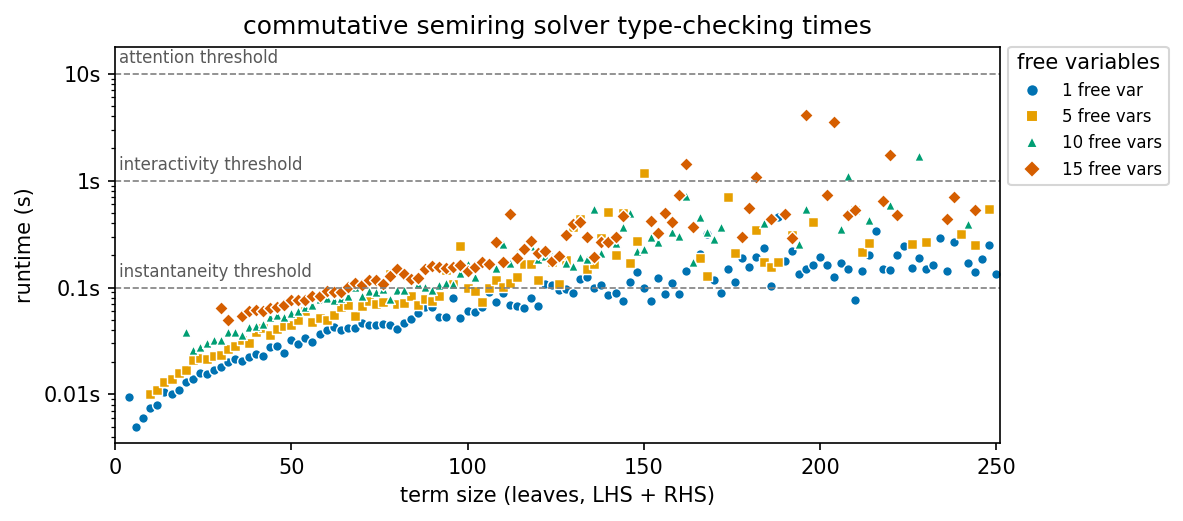
\includegraphics[width=0.8\textwidth]{images/benchmark_semiring.png}
    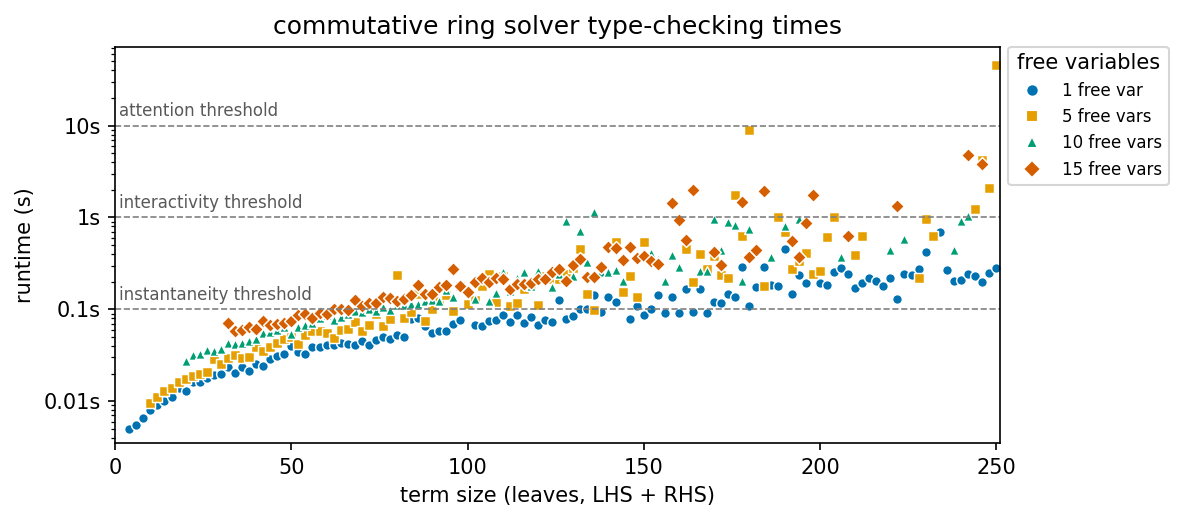
\includegraphics[width=\textwidth]{images/benchmark_ring.png}
  \end{figure}
\end{frame}


\begin{frame}[t]{Equational theories}
  \pause
  \structure{Presentation} $\TT = (\Sigma_\TT, \Ax_\TT)$
  \begin{itemize}
    \item \emph{signature} $\Sigma_\TT$: operation symbols with arity.
    \item \emph{axioms} $\Ax_\TT$: axioms between $\Sigma_\TT$-terms.
  \end{itemize}
  A \emph{$\TT$-model} interprets the operations and satisfies the axioms.

  \pause
  \vspace{0.2cm}
  \structure{Example: monoids}
  \begin{itemize}
    \item operations: $\{(\cdot) : 2,\; 1 : 0\}$
    \item axioms:
    \begin{align*}
      x, y, z &\vdash x \cdot (y \cdot z) = (x \cdot y) \cdot z &\text{associativity}\\
      x &\vdash 1 \cdot x = x &\text{left neutrality}\\
      x &\vdash x \cdot 1 = x &\text{right neutrality}\\
    \end{align*}
    \item $(\N, (+), 0)$, $(\N, (\times), 1)$ are models.
  \end{itemize}
\end{frame}

\begin{frame}[t]{The distributive combination of theories}
  \begin{columns}
    \column{0.5\textwidth}
    \structure{Additive part}

    Presentation $\AA = \la \Sigma_\AA, \Ax_\AA \ra$

    \column{0.5\textwidth}
    \structure{Multiplicative part}

    Presentation $\MM = \la \Sigma_\MM, \Ax_\MM \ra$
  \end{columns}
  \vspace{0.5cm}
  \structure{Distributive combination} $\MM \dist \AA$

  $\Sigma_{\MM\dist\AA} = \Sigma_\AA \sqcup \Sigma_\MM$
  \begin{align*}
    \Ax_{\MM\dist\AA} &= \Ax_\AA \sqcup \Ax_\MM\\
    &\sqcup \text{ distributivity axioms of every $\MM$-operation over every $\AA$-operation}
  \end{align*}

  \pause
  \structure{Example}

  Semiring = monoid $\dist$ commutative monoid

  Distributivity axioms:
  \begin{gather*}
    x, y, z \vdash x \cdot (y + z) = (x \cdot y) + (x \cdot z) \qquad x, y, z \vdash (x + y) \cdot z = (x \cdot z) + (y \cdot z)\\
    x \vdash x \cdot 0 = 0 \qquad x \vdash 0 \cdot x = 0
  \end{gather*}
\end{frame}

\begin{frame}[t, fragile]{Free algebras}
  Presentation $\TT$, set of variables $X$.

  \structure{Free $\TT$-model over $X$ $\la F_\TT X, \eta^\TT \ra$:} ``most general'' $\TT$-model generated by $X$.

  \medskip

  \structure{Intuition:}
  \begin{itemize}
    \item elements of $F_\TT X$ = $\TT$-expressions modulo the axioms of $\TT$
    \item the \emph{unit} $\eta^\TT : X \to \underbrace{\underline{F_\TT X}}_{\text{carrier set}}$ embeds the variables in $X$ in $F_\TT X$
    % \item $F_\TT X$ provides normal forms
  \end{itemize}

  \medskip
  \pause
  \structure{Universal property:}

  for every $\TT$-model $A$ and function $e : X \to \underline{A}$, there exists a unique $\TT$-homomorphism $h : F_\TT X \to A$ such that:
  \[\begin{tikzcd}
	X & {\underline{F_\TT X}} \\
	& \underline{A}
	\arrow["{\eta^\TT}", from=1-1, to=1-2]
	\arrow[""{name=0, anchor=center, inner sep=0}, "e"', from=1-1, to=2-2]
	\arrow["\underline{h}", from=1-2, to=2-2]
	\arrow["{=}"{description, pos=0.6}, draw=none, from=0, to=1-2]
\end{tikzcd}\]
\end{frame}

\begin{frame}{Free algebras}
  \structure{Example: free monoid over $X$}
  \begin{itemize}
    \item $\underline{F_\Mon X} := \List X \qquad u \cdot v := u \concat v \qquad 1 := [] \qquad \eta^\Mon \; x := [x]$
    \item $\Monoid$-model $A$, function $e : X \to \underline{A}$\\ $\Rightarrow$ unique monoid homomorphism $h$: $$\underline{h}\ [x_1, \dots, x_n] := 1 \cdot (e\; x_1) \cdot \ldots \cdot (e\; x_n)$$ $\underline{h} (\eta^\Mon\; x) = \underline{h}\ [x] = 1 \cdot (e\; x) = e\; x$
    % since $A$ is a $\Monoid$-model
  \end{itemize}

  \bigskip
  \pause

  \structure{Example: free commutative monoid over $X$}
  \begin{itemize}
    \item $\underline{F_\CMon X} := \Bag X \qquad u + v := u \uplus v \qquad 0 := \Lbag \Rbag \qquad \eta^\CMon\; x := \Lbag x : 1 \Rbag$
    \item $\CMonoid$-model $A$, function $e : X \to \underline{A}$\\ $\Rightarrow$ unique commutative monoid homomorphism $h$: $$\underline{h}\ \mathrm{bag} := 0 + \sum_{(x : n) \in \mathrm{bag}} n \cdot (e\; x) \qquad \text{notation: } n \cdot x := \underbrace{x + \ldots + x}_{n \text{ times}}$$ $\underline{h} (\eta^\CMon\; x) = \underline{h}\ \Lbag x : 1 \Rbag = 0 + (e\; x) = e\; x$ 
    % since $A$ is a $\CMonoid$-model
  \end{itemize}
\end{frame}

\begin{frame}[t]{Free algebras and normalisation}
  \begin{theorem}[Extensional normalisation, informally]
    Let $\la F_\TT X, \eta^\TT \ra$ be a free $\TT$-model over the set $X$, and $s, t$ be expressions with variables from $X$.

    The equation $s = t$ is valid in every $\TT$-model iff their interpretations in $F_\TT X$ are equal.
  \end{theorem}
  \vspace{0.3cm}
  \pause
  \structure{Example: monoids}

  The equation $$x, y \vdash x \cdot (y \cdot 1) = 1 \cdot (x \cdot y)$$ holds in every monoid since $$[x] \concat ([y] \concat []) = [x,\; y] = [] \concat ([x] \concat [y])$$
\end{frame}


% \section{Contribution: free algebra for the distributive combination of theories}

\begin{frame}[t]{Free algebra for the distributive combination}
  \begin{columns}[t]
    \column{0.5\textwidth}
    \structure{Free additive algebra}
    
    \begin{itemize}
      \item $\AA$ \emph{commutative}:
      
      every operation commutes with every other operation
      \item $F_\AA = \la F_\AA X, \eta^\AA \ra$
    \end{itemize}
    
    \column{0.5\textwidth}
    \structure{Free multiplicative algebra}

    \begin{itemize}
      \item $\MM$ arbitrary
      \item $F_\MM = \la F_\MM X, \eta^\MM \ra$
    \end{itemize}
  \end{columns}
  \vspace{0.5cm}
  
  \structure{Free distributive combination algebra (hypothesis)}
  \begin{itemize}
    \item $\underline{F_{\MM\dist\AA}X} := \underline{F_\AA \underline{F_\MM X}}$
    \item additive operations from $F_\AA \underline{F_\MM X}$
    \item ``lifted'' multiplicative operations of $F_\MM X$
    \item $\eta^{\MM\dist\AA} := \eta^\AA \circ \eta^\MM$
  \end{itemize}
\end{frame}

\begin{frame}[t]{Free algebra for the distributive combination}
  % \structure{Free distributive combination algebra (hypothesis)}
  % \begin{itemize}
  %   \item $\underline{F_{\MM\dist\AA}X} := \underline{F_\AA \underline{F_\MM X}}$
  %   \item additive operations from $F_\AA \underline{F_\MM X}$
  %   \item ``lifted'' multiplicative operations of $F_\MM X$
  %   \item $\eta^{\MM\dist\AA} := \eta^\AA \circ \eta^\MM$
  % \end{itemize}

  % \vspace{0.3cm}
  \structure{Example: semirings}
  \begin{itemize}
    \item $\underline{F_{\Mon\dist\CMon}X} := \Bag \List X$
    \item $u + v := u \uplus v$
    \item lifted multiplication:
    \begin{gather*}
      2xy \cdot (3xz + t) = 6xyxz + 2xyt\\
      \Lbag [x, y] : 2 \Rbag \cdot \Lbag [x, z] : 3,\ [t] : 1 \Rbag = \Lbag [x, y, x, z] : 6, [x, y, t] : 2 \Rbag\\
      u \cdot v := \biguplus_{(l_1 : n_1) \in u} \biguplus_{(l_2 : n_2) \in v} \Lbag l_1 \concat l_2 : n_1 \times n_2 \Rbag
    \end{gather*}
    \item $\eta^{\Mon\dist\CMon} x := \Lbag [x] : 1 \Rbag$
    \item $x \in \Bag\List X$, $\displaystyle\underline{h}\ x := 0 + \sum_{([x_1, \dots, x_n] : n) \in x} n \cdot \bigl( 1 \cdot (e\; x_1) \cdot \ldots \cdot (e\; x_n) \bigr)$
  \end{itemize}
\end{frame}

\begin{frame}[t]{Failure: no-go results}
  \parencite{nogo_distributive_law}: the previous construction doesn't work if any of these 3 hypotheses hold:
  \begin{enumerate}
    \item $\MM$ has an idempotent operator\\ (i.e. there exists $(\ast : 2) \in \Sigma_\MM$ such that $x \vdash x \ast x = x$ holds)
    \item $\AA$ has two or more distinct constants
    \item $a, b, c, d \vdash (a \ast b) \ast (c \ast d) = (a \ast c) \ast (b \ast d)$ does not hold for every $(\ast : 2) \in \Sigma_\AA$ 
  \end{enumerate}
  \pause
  \medskip
  \begin{columns}[t]
    \column{0.5\textwidth}
    \structure{Free additive algebra}
    
    \begin{itemize}
      \item $\AA$ \textbf{commutative}:
      
      every operation commutes with every other operation
    \end{itemize}
    
    \column{0.5\textwidth}
    \structure{Free multiplicative algebra}

    \begin{itemize}
      \item $\MM$ \only<1-3>{arbitrary}\only<4->{\sout{arbitrary} \emph{affine}}
    \end{itemize}
  \end{columns}

  \bigskip
  2. and 3. are false under the commutativity hypothesis

  \pause
  \medskip
  \structure{Problem:} What about 1.? \pause $\Rightarrow$ \emph{affinity} hypothesis for $\MM$
\end{frame}


\begin{frame}[t]{Corrected theorem}
  \structure{Affine presentation}
  \begin{itemize}
    \item $\TT$ presentation
    \item such that in every axiom, each variable appears at most once \textbf{on each side}
  \end{itemize}

  \structure{Examples:}

  \begin{itemize}
    \item $x, y \vdash x + y = y + x$ is affine
    \item $x \vdash x \cdot 0 = 0$ is affine
    \item $x \vdash x \vee x = x$ is \emph{not} affine
  \end{itemize}

  Semigroups, monoids, groups: all affine theories

  \pause
  \begin{theorem}[Informally stated]
    If the additive theory is commutative and the multiplicative theory is affine, then the free algebra of the distributive combination is given by composition of the component free algebras.
  \end{theorem}
\end{frame}

% \begin{frame}{Practical payoff}
%   $$\begin{pmatrix}
%     commutative\ semigroups\\
%     commutative\ monoids\\
%     Abelian\ groups
%   \end{pmatrix} \times \begin{pmatrix}
%     semigroups\\
%     monoids\\
%     groups
%   \end{pmatrix} \times \begin{pmatrix}
%     mere\\
%     commutative
%   \end{pmatrix} \times \begin{pmatrix}
%     mere\\
%     involutive
%   \end{pmatrix}$$

%   This already yields 28 non-trivial modular solvers.

%   \pause
%   \begin{figure}
%     \centering
%     % 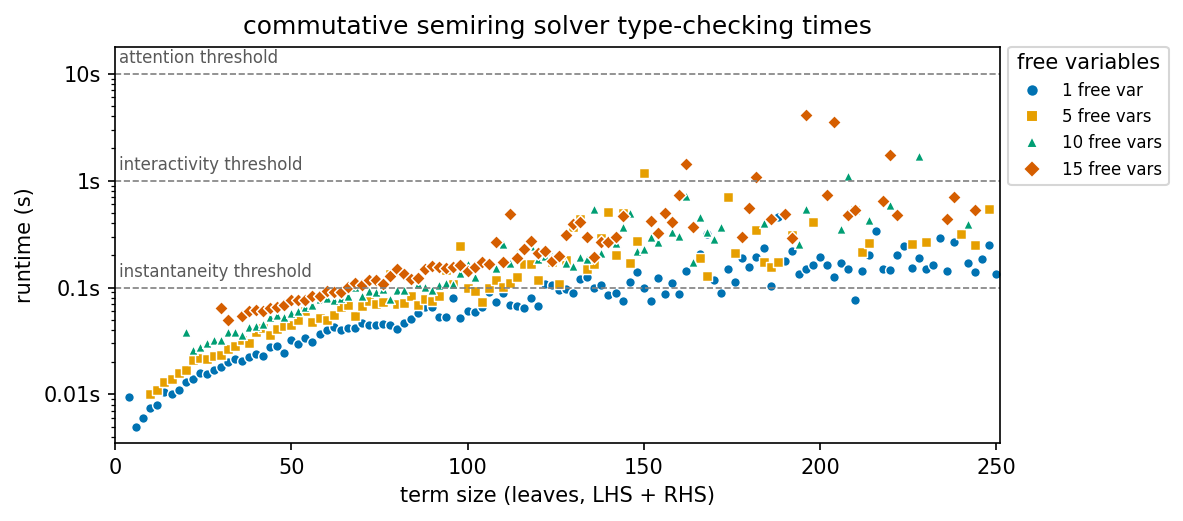
\includegraphics[width=0.8\textwidth]{images/benchmark_semiring.png}
%     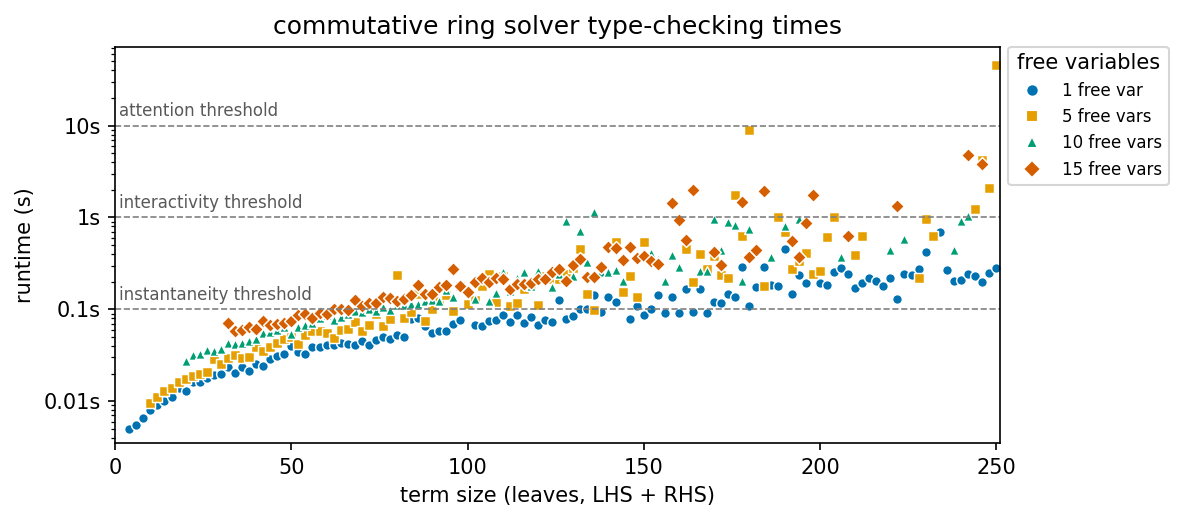
\includegraphics[width=0.8\textwidth]{images/benchmark_ring.png}
%   \end{figure}
% \end{frame}

\begin{frame}{Possible extensions}
  \begin{itemize}
    \item \structure{free extensions}
    
    like free algebras but also embed constants from an existing model
    \pause
    \item \structure{full mechanisation}
    
    complete the Idris 2 proof of the main theorem
    \pause
    \item \structure{optimality of the hypothesis}
    
    something weaker than affinity?
    % \pause
    % \item \structure{proof extraction}
    
    % implement printers for the distributive combination 
    
    % $\Rightarrow$ proof pretty-printing
    \pause
    \item \structure{multi-sorted theories}
    
    examples: non-square matrices, linear transformations, modules
  \end{itemize}
\end{frame}

\begin{frame}{Conclusion}
  \begin{itemize}
    \item \structure{free algebras:}\\ normal forms modulo axioms
    \item \structure{solving:}\\ extensional normalisation
    \item \structure{distributive combination of theories:}\\ disjoint union + distributivity axioms
    \item \structure{free algebra for the distributive combination of theories:}\\ composition of the component free algebras \begin{itemize}
      \item commutative additive theory
      \item affine multiplicative theory
    \end{itemize}
    \item \structure{modularity:}\\ already 28 non-trivial solvers
  \end{itemize}
\end{frame}

\appendix
\backupbegin

\section*{Appendices}

\begin{frame}
	\sectionpage
\end{frame}

\begin{frame}{Appendix outline}
  % Source - https://tex.stackexchange.com/a/368398
% Posted by samcarter_is_at_topanswers.xyz, modified by community. See post 'Timeline' for change history
% Retrieved 2026-08-23, License - CC BY-SA 3.0

\tableofcontents[sectionstyle=show/hide, subsectionstyle=show/show/hide]

\end{frame}

\subsection{Category theory}

\begin{frame}
	\subsectionpage
\end{frame}

\begin{frame}[fragile]{Monads}
  A \emph{monad} on a category $\mathcal C$ is a triple $(T,\eta,\mu)$ where:
  \begin{itemize}
    \item $T:\mathcal C\to\mathcal C$
    \item $\eta:1_{\mathcal C}\Rightarrow T$
    \item $\mu:T^2\Rightarrow T$
  \end{itemize}
  and such that the following diagrams commute:
  \[
  \begin{tikzcd}
    T \arrow[r, "T\eta"] \arrow[d, "\eta T"'] \arrow[equal, dr, ""] & T^2 \arrow[d, "\mu"] \\
    T^2 \arrow[r, "\mu"'] & T
  \end{tikzcd}
  \quad\quad
  \begin{tikzcd}
    T^3 \arrow[r, "T\mu"] \arrow[d, "\mu T"'] & T^2 \arrow[d, "\mu"] \\
    T^2 \arrow[r, "\mu"'] & T
  \end{tikzcd}
  \]
\end{frame}

\begin{frame}[fragile]{Distributive laws}
  A \emph{distributive law} of $(T, \eta^T, \mu^T)$ over $(S, \eta^S, \mu^S)$ is a natural transformation $\lambda : TS \Rightarrow ST$ such that the following diagrams commute:
  \[
  \begin{tikzcd}
                          & T \arrow[ld, "T\eta^S"'] \arrow[rd, "\eta^ST"] &    \\
TS \arrow[rr, "\lambda"'] &                                                & ST
\end{tikzcd}
  \quad\quad
  \begin{tikzcd}
                          & S \arrow[ld, "\eta^TS"'] \arrow[rd, "S\eta^T"] &    \\
TS \arrow[rr, "\lambda"'] &                                                & ST
\end{tikzcd}
  \]
  \[
  \begin{tikzcd}
    T^2 S \arrow[r, "T\lambda"] \arrow[d, "\mu^T S"'] & TST \arrow[r, "\lambda T"] & ST^2 \arrow[d, "S\mu^T"] \\
    TS \arrow[rr, "\lambda"'] & & ST
  \end{tikzcd}
  \quad\quad
  \begin{tikzcd}
    TS^2 \arrow[r, "\lambda S"] \arrow[d, "T\mu^S"'] & STS \arrow[r, "S\lambda"] & S^2T \arrow[d, "\mu^S T"] \\
    TS \arrow[rr, "\lambda"'] & & ST
  \end{tikzcd}
  \]
\end{frame}

% \begin{frame}[fragile]{Pullback used in the proof of the main theorem}
%   \[
% % https://q.uiver.app/#q=WzAsNCxbMCwwLCJcXE1vZChcXG1hdGhmcmFrIFQgXFx0cmlhbmdsZWxlZnRcXG1hdGhjYWwgQSwgXFxTZXQpIl0sWzAsMSwiXFxNb2QoXFxtYXRoY2FsIE0sIFxcU2V0KSJdLFsxLDEsIlxcTW9kKFxcbWF0aGNhbCBPLCBcXGxhIFxcU2V0LCBcXHByb2QgXFxyYSkiXSxbMSwwLCJcXE1vZChcXG1hdGhjYWwgTywgXFxNdWx0aShcXG1hdGhjYWwgQSwgXFxTZXQpKSJdLFszLDIsIlxcTW9kKFxcbWF0aGNhbCBPLCBcXHVuZGVybGluZXstfSkiXSxbMCwzLCJcXHVuZGVybGluZXstfV97XFxtYXRoY2FsIE8gXFx0cmlhbmdsZWxlZnQgXFxtYXRoY2FsIEF9Il0sWzEsMiwiXFxNb2QoXFxtYXRoZnJhayBULCBcXFNldCkiLDJdLFswLDEsIlxcdW5kZXJsaW5ley19X3tcXG1hdGhjYWwgTX0iLDJdLFswLDYsIiIsMSx7ImxldmVsIjoxLCJzdHlsZSI6eyJuYW1lIjoiY29ybmVyIn19XV0=&macro_url=https%3A%2F%2Fraw.githubusercontent.com%2FS-c-r-a-t-c-h-y%2Fsemiring-solvers%2Frefs%2Fheads%2Fmain%2Fmacros.sty
% \begin{tikzcd}
% 	{\Mod(\mathfrak T \triangleleft\mathcal A, \Set)} & {\Mod(\mathcal O, \Multi(\mathcal A, \Set))} \\
% 	{\Mod(\mathcal M, \Set)} & {\Mod(\mathcal O, \la \Set, \prod \ra)}
% 	\arrow["{\underline{-}_{\mathcal O \triangleleft \mathcal A}}", from=1-1, to=1-2]
% 	\arrow["{\underline{-}_{\mathcal M}}"', from=1-1, to=2-1]
% 	\arrow["{\Mod(\mathcal O, \underline{-})}", from=1-2, to=2-2]
% 	\arrow[""{name=0, anchor=center, inner sep=0}, "{\Mod(\mathfrak T, \Set)}"', from=2-1, to=2-2]
% 	\arrow["\lrcorner"{anchor=center, pos=0.125}, draw=none, from=1-1, to=0]
% \end{tikzcd}
% \]
% \end{frame}

\subsection{Universal algebra}

\begin{frame}
	\subsectionpage
\end{frame}

\begin{frame}{Formal syntax}
  \structure{Finitary signature} $\Sigma = (\op \Sigma,\; \arity_\Sigma)$

  describes the operators of a theory
  \begin{itemize}
    \item \emph{operator} set: $\op\Sigma \in \Set$ 
    \item \emph{arity} assignment: $\arity_\Sigma : \op\Sigma \to \N$
  \end{itemize}

  \vspace{0.5cm}
  \structure{Example: monoid signature $\Sigma_\Mon$}
  \begin{itemize}
    \item $\op\Sigma_\Mon := \{(\cdot), 1\}$
    \item $\arity_{\Sigma_\Mon} (\cdot) := 2$, i.e, $(\cdot)$ is a binary operator
    \item $\arity_{\Sigma_\Mon} 1 := 0$, i.e, $1$ is a constant
  \end{itemize}
  Written succintly: $\Sigma_\Mon := \{(\cdot) : 2,\; 1 : 0\}$
\end{frame}

\begin{frame}{Interpretation}
  \structure{Algebra} $A = (\underline{A},\; A \brak{-})$ \structure{over a signature $\Sigma$}
  \begin{itemize}
    \item \emph{carrier} set: $\underline{A} \in \Set$
    \item \emph{operations} or \emph{interpretations}: $A\brak{f} : \underline{A}^n \to \underline{A}$ for all $(f : n) \in \Sigma$
  \end{itemize}

  \vspace{0.5cm}
  \structure{Example: monoids}
  \begin{itemize}
    \item $(\N, (+), 0)$
    \item $(\N, (\cdot), 1)$
    \item $(\N, \max, 0)$
    \item $(\C, (+), 0)$
    \item $(\C, (\cdot), 1)$
  \end{itemize}
\end{frame}

\begin{frame}{Structure-preserving maps}
  \structure{Homomorphism} $h : A \to B$

  between $\Sigma$-algebras $A, B$:
  \begin{itemize}
    \item function $\underline h : \underline{A} \to \underline{B}$
    \item such that: $$B \brak{f}\bigr(h(a_1), \ldots, h(a_n)\bigl) = h\bigr(A \brak{f}(a_1, \ldots, a_n)\bigl)$$ for all $(f : n) \in \Sigma$ and $a_1, \dots, a_n \in \underline{A}$
  \end{itemize}

  \vspace{0.5cm}
  \structure{Example: complex conjugation}
  \begin{itemize}
    \item $\bar{z_1 + z_2} = \bar{z_1} + \bar{z_2}, \quad \bar{0} = 0$
    \item $\bar{z_1 \cdot z_2} = \bar{z_1} \cdot \bar{z_2}, \quad \bar{1} = 1$
  \end{itemize}
\end{frame}

\begin{frame}{Abstract syntax}
  \structure{$\Term_\Sigma X$:} terms over signature $\Sigma$ and variable set $X$

  $$\dfrac{x \in X}{x \in \Term_\Sigma X} \qquad \dfrac{t_i \in \Term_\Sigma X \quad (\op : n) \in \Sigma}{\op(t_1, \dots, t_n) \in \Term_\Sigma X}$$

  \vspace{0.3cm}
  \structure{Term folding} $A\brak{t} e$
  \begin{itemize}
    \item $\Sigma$-algebra $A$
    \item \emph{environment} $e : X \to \underline A$ \smash{\raisebox{.5\dimexpr\baselineskip+\itemsep+\parskip}{$\left.\rule{0pt}{.5\dimexpr2\baselineskip+3\itemsep+3\parskip}\right\}\mathit{\Sigma-\textit{algebra over } X}$}}
  \end{itemize}
  Inductively:
  $$A \brak{x} e := e\; x \qquad A \brak{\op(t_1, \dots, t_n)} e := A \brak{\op} \bigl(A \brak{t_1} e, \dots, A \brak{t_n} e\bigr)$$
  \structure{Example: monoid}
  \begin{itemize}
    \item term $t := x \cdot (y \cdot 1)$
    \item interpretation  with $e := \{x \mapsto 2,\; y \mapsto 3\}$ in $A := (\N, (+), 0)$
    $$A\brak{x \cdot (y \cdot 1)} = 2 + (3 + 0) = 5$$
  \end{itemize}
\end{frame}

% this abstract syntax lets us define equations and talk about validity of equations

\begin{frame}{Validity}
  \structure{Equation} $X \vdash_\Sigma \ell = r$ \structure{over signature $\Sigma$}
  \begin{itemize}
    \item set $X$
    \item terms $\ell, r \in \Term_\Sigma X$
  \end{itemize}

  \vspace{0.3cm}
  \structure{Satisfaction} $\la A, e \ra \models (X \vdash \ell = r)$

  by $\Sigma$-algebra over $X$ $\la A, e \ra$: $$A\brak{\ell} e = A\brak{r} e$$

  \structure{Validity} $A \models (X \vdash \ell = r)$

  in algebra $A$:
  $$\forall e : X \to \underline{A},\quad \la A, e \ra \models (X \vdash \ell = r)$$
\end{frame}

\begin{frame}[t]{Validity}
  \structure{Satisfaction} $\la A, e \ra \models (X \vdash \ell = r)$

  by $\Sigma$-algebra over $X$ $\la A, e \ra$: $$A\brak{\ell} e = A\brak{r} e$$

  \structure{Validity} $A \models (X \vdash \ell = r)$

  in algebra $A$:
  $$\forall e : X \to \underline{A},\quad \la A, e \ra \models (X \vdash \ell = r)$$

  \structure{Example:}
  \begin{itemize}
    \item $\la A := (\N, (+), 0),\; e := \{x \mapsto 2,\; y \mapsto 3\} \ra$ satisfies $$x, y \vdash x \cdot (y \cdot 1) = 1 \cdot (x \cdot y)$$
    since $$2 + (3 + 0) = 5 = 0 + (2 + 3)$$
  \end{itemize}
\end{frame}

% we'll see later that this equation (the example one) is valid in all monoids

\begin{frame}{Varieties of algebras}
  \structure{Presentation} $\TT = (\Sigma_\TT,\; \Ax_\TT)$
  \begin{itemize}
    \item signature $\Sigma_\TT$
    \item set $\Ax_\TT$ of $\Sigma_\TT$-equations, the \emph{axioms}
  \end{itemize}
  \emph{$\TT$-model}: $\Sigma_\TT$-algebra validating every axiom in $\TT$: $A \models (X \vdash \ell = r) \in \Ax_\TT$

  \vspace{0.5cm}
  \structure{Example: monoids}
  
  $\Monoid$ presentation $:= (\Sigma_\Mon,\; \Ax_\Monoid)$ with the axioms
  \begin{align*}
    x, y, z &\vdash x \cdot (y \cdot z) = (x \cdot y) \cdot z &\text{associativity}\\
    x &\vdash 1 \cdot x = x &\text{left neutrality}\\
    x &\vdash x \cdot 1 = x &\text{right neutrality}\\
  \end{align*}
  monoids are $\Monoid$-models
\end{frame}

\begin{frame}[t]{Free algebras}
  \structure{Free $\TT$-model over $X$} $\la F_\TT X,\; \eta^\TT \ra$
  \begin{itemize}
    \item $\TT$-model $F_\TT X$
    \item environment $\eta^\TT$ called the \emph{unit}
    \item \emph{universal property}:
    
    every $\TT$-model over $X$ $\la A,\; e \ra$ uniquely defines \begin{itemize}
      \item a homomorphism $h : F_\TT X \to A$
      \item that extends $e$ along $\eta^\TT$: $e = h \circ \eta^\TT$
    \end{itemize}
  \end{itemize}

  \structure{Example: free monoid over $X$}
  \begin{itemize}
    \item $\underline{F_\Mon X} := \List X \qquad u \cdot v := u \concat v \qquad 1 := [] \qquad \eta^\Mon \; x := [x]$
    \item for every $\Monoid$-model over $X$ $\la A, e \ra$, a unique monoid homomorphism $h$: $$\underline{h}\ [x_1, \dots, x_n] := 1 \cdot (e\; x_1) \cdot \ldots \cdot (e\; x_n)$$ $\underline{h} (\eta^\Mon\; x) = \underline{h}\ [x] = 1 \cdot (e\; x) = e\; x$
    since $F_\Mon X$ is a $\Monoid$-model
  \end{itemize}
\end{frame}

\begin{frame}[t]{Free algebras}
  \structure{Free $\TT$-model over $X$} $\la F_\TT X,\; \eta^\TT \ra$
  \begin{itemize}
    \item $\TT$-model $F_\TT X$
    \item environment $\eta^\TT$ called the \emph{unit}
    \item \emph{universal property}:
    
    every $\TT$-model over $X$ $\la A,\; e \ra$ uniquely defines \begin{itemize}
      \item a homomorphism $h : F_\TT X \to A$
      \item that extends $e$ along $\eta^\TT$: $e = h \circ \eta^\TT$
    \end{itemize}
  \end{itemize}

  \structure{Example: free commutative monoid over $X$}
  \begin{itemize}
    \item $\underline{F_\CMon X} := \Bag X \qquad u \cdot v := u \uplus v \qquad 1 := \Lbag \Rbag \qquad \eta^\CMon\; x := \Lbag x : 1 \Rbag$
    \item for every $\CMonoid$-model over $X$ $\la A, e \ra$, a unique commutative monoid homomorphism $h$: $$\underline{h}\ \mathrm{bag} := 1 \cdot \sum_{(x : n) \in \mathrm{bag}} n \cdot (e\; x) $$ $\underline{h} (\eta^\CMon\; x) = \underline{h}\ \Lbag x : 1 \Rbag = 1 \cdot (e\; x) = e\; x$ 
    % since $F_\CMonoid X$ is a $\CMonoid$-model
  \end{itemize}
\end{frame}

% but why is all of this relevant to our problem, which we recall was solving some equations in some theories
% the answer lies in the following theorem: free algebras can be used to prove equalities

\begin{frame}[t]{Free algebras and normalisation}
  \begin{theorem}[extensional normalisation]
    Let $\la F_\mathcal{T}X, \env \ra$ be a free $\mathcal{T}$-model, and let $X \vdash \ell = r$ be an equation in context. The following are equivalent:
    \begin{enumerate}
      \item The unit satisfies the equation: $\la F_\mathcal{T}X, \env \ra \models (X \vdash \ell = r)$
      \item The free algebra validates the equation: $F_\mathcal{T}X \models (X \vdash \ell = r)$
      \item Every $\mathcal{T}$-model $A$ validates the equation: $A \models (X \vdash \ell = r)$
    \end{enumerate}
  \end{theorem}
  \begin{proof}
    3. $\imp$ 2. and 2. $\imp$ 1. hold by definition.
  
    1. $\imp$ 3. is deduced from the universal property of the fral.
  \end{proof}
\end{frame}

\begin{frame}[t]{Free algebras and normalisation}
  \begin{theorem}[extensional normalisation]
    Let $\la F_\mathcal{T}X, \env \ra$ be a free $\mathcal{T}$-model, and let $X \vdash \ell = r$ be an equation in context. The following are equivalent:
    \begin{enumerate}
      \item The unit satisfies the equation: $\la F_\mathcal{T}X, \env \ra \models (X \vdash \ell = r)$
      \item The free algebra validates the equation: $F_\mathcal{T}X \models (X \vdash \ell = r)$
      \item Every $\mathcal{T}$-model $A$ validates the equation: $A \models (X \vdash \ell = r)$
    \end{enumerate}
  \end{theorem}

  \structure{Example: monoids}

  The equation $$x, y \vdash x \cdot (y \cdot 1) = 1 \cdot (x \cdot y)$$ holds in every monoid since $$[x] \concat ([y] \concat []) = [x,\; y] = [] \concat ([x] \concat [y])$$
\end{frame}

\begin{frame}[t]{Commutative theories}
  \structure{Commutative theory}
  \begin{itemize}
    \item $\TT$ presentation
    \item such that every operator commutes with every other operator: $$f \begin{pmatrix}
  g(x_{11}, \dots, x_{1m})\\
  \vdots\\
  g(x_{n1}, \dots, x_{nm})
\end{pmatrix} = g \lp
  f \begin{pmatrix}
    x_{11}\\
    \vdots\\
    x_{n1}
  \end{pmatrix},\ \cdots\ ,f \begin{pmatrix}
    x_{1m}\\
    \vdots\\
    x_{nm}
  \end{pmatrix}
\rp$$ holds in every $\TT$-model for every $(f : n) \in \Sigma_\TT$, $(g : m) \in \Sigma_\TT$
  \end{itemize}
  
  \vspace{0.3cm}
  \structure{Example: monoids}
  
  The equations are:
  $$(x \cdot y) \cdot (z \cdot w) = (x \cdot z) \cdot (y \cdot w) \qquad 1 \cdot 1 = 1 \qquad 1 = 1$$

  The theory of commutative monoids is commutative.
\end{frame}

\begin{frame}[t]{Affine theories}
  \structure{Affine theory}
  \begin{itemize}
    \item $\TT$ presentation
    \item such that in every axioms, each variable appears at most once
  \end{itemize}

  \vspace{0.3cm}
  \structure{Examples:}

  \begin{itemize}
    \item $x, y \vdash x + y = y + x$ is affine
    \item $x \vdash x \cdot 0 = 0$ is affine
    \item $x \vdash x \vee x = x$ is \emph{not} affine
  \end{itemize}

  Semigroups, monoids, groups: all affine theories
\end{frame}

\begin{frame}[fragile, t]{Extensions and morphisms of extensions}
  \structure{Extension of $A$ by $X$} $\la B, h, e \ra$

  where $A$ is a $\TT$-model and $X$ a set.
  \begin{itemize}
    \item $\TT$-model $B$
    \item homomorphism of $\TT$-models $h : A \to B$
    \item function $e : X \to \underline B$ 
  \end{itemize}

  \vspace{0.5cm}
  \structure{Morphism of extensions} $h : b_1 \to b_2$ 
  
  between extensions of $A$ by $X$ $b_1 = \la B_1, h_1, e_1 \ra$ and $b_2 = \la B_2, h_2, e_2 \ra$.
  \begin{itemize}
    \item homomorphism of $\TT$-models $h : B_1 \to B_2$
    \item such that the following diagram commutes: \[\begin{tikzcd}[sep=small]
    & {B_1} & \\
    X && A \\
    & {B_2}
    \arrow["h", from=1-2, to=3-2]
    \arrow["{e_1}", from=2-1, to=1-2]
    \arrow["{e_2}"', from=2-1, to=3-2]
    \arrow["{h_1}"', from=2-3, to=1-2]
    \arrow["{h_2}", from=2-3, to=3-2]
  \end{tikzcd}\]
  \end{itemize}
\end{frame}

\begin{frame}[t]{Free extensions}
  \structure{Free extension of $A$ by $X$} $\la A[X], \sta, \dyn \ra$
  \begin{itemize}
    \item extension of $A$ by $X$ $\la A[X], \sta, \dyn \ra$
    \item \emph{universal property}:
    
    every extension of $A$ by $X$ $\la B, h, e \ra$ uniquely defines a morphism of extensions $[B, h, e] : \la A[X], \sta, \dyn \ra \to \la B, h, e \ra$
  \end{itemize}

  \vspace{0.5cm}
  \structure{Example: commutative monoids}

  $A$ commutative monoid, $X = \{x_1, x_2, x_3\}$

  \begin{gather*}
    A[X] := \underline{A} \times \N^3\\
    \la a, \la k_{11}, k_{12}, k_{13} \ra \ra + \la b, \la k_{21}, k_{22}, k_{23} \ra \ra := \la a + b, \la k_{11} + k_{21}, k_{12} + k_{22}, k_{13} + k_{23} \ra \ra\\
    0 := \la 0, \la 0, 0, 0 \ra \ra \qquad \sta\; a := \la a, \la 0, 0, 0 \ra \ra\\
    \dyn\; x_1 := \la 0, \la 1, 0, 0 \ra\ra \qquad \dyn\; x_i := \dots\\
    [B, h, e]\; \la a, \la k_1, k_2, k_3 \ra \ra := h\; a + k_1 \cdot e\; x_1 + k_2 \cdot e\; x_2 + k_3 \cdot e\; x_3
  \end{gather*}
\end{frame}

\subsection{Proof}

\begin{frame}
	\subsectionpage
\end{frame}

\begin{frame}[t]{Proof idea}

  \structure{Goal:} construct $F_{\MM\dist\AA} X$ from $F_\MM X$ and $F_\AA X$

  \begin{enumerate}
    \item Start with $F_\MM X$
    \item Apply the free additive algebra: $F_\AA(F_\MM X)$
    
    % This gives the candidate carrier.
    \item The additive operations are already there.
    % The hard part is to lift the multiplicative operations so that they distribute over the additive ones.
    \item Use the commutativity of $\AA$ to lift the multiplicative operations.
    \item Use the affinity of $\MM$ to prove that the lifted operations still satisfy the axioms of $\MM$.
    \item The universal properties of the two free constructions combine to show that the resulting model is free.
  \end{enumerate}

  \medskip

  \structure{Underlying concepts:} 
  
  operads/translations, multicategories, an adjunction used for lifting, a pullback description of models of the distributive combination
\end{frame}

\begin{frame}[t]{Lifting of the multiplicative operations}
  \begin{theorem}
  Let $\TT$ be a theory. The forgetful multi-functor $\underline- :
  \Multi(\TT, \Set) \to \la \Set,\; \prod \ra$ has a left adjoint iff $\TT$
  is commutative.
\end{theorem}
\end{frame}

\begin{frame}[fragile]{Pullback square}

$\AA$ and $\MM$ theory, $\OO$ operad, $T : \OO \to \MM$ translation

\[
% https://q.uiver.app/#q=WzAsNCxbMCwwLCJcXE1vZChcXG1hdGhmcmFrIFQgXFx0cmlhbmdsZWxlZnRcXG1hdGhjYWwgQSwgXFxTZXQpIl0sWzAsMSwiXFxNb2QoXFxtYXRoY2FsIE0sIFxcU2V0KSJdLFsxLDEsIlxcTW9kKFxcbWF0aGNhbCBPLCBcXGxhIFxcU2V0LCBcXHByb2QgXFxyYSkiXSxbMSwwLCJcXE1vZChcXG1hdGhjYWwgTywgXFxNdWx0aShcXG1hdGhjYWwgQSwgXFxTZXQpKSJdLFszLDIsIlxcTW9kKFxcbWF0aGNhbCBPLCBcXHVuZGVybGluZXstfSkiXSxbMCwzLCJcXHVuZGVybGluZXstfV97XFxtYXRoY2FsIE8gXFx0cmlhbmdsZWxlZnQgXFxtYXRoY2FsIEF9Il0sWzEsMiwiXFxNb2QoXFxtYXRoZnJhayBULCBcXFNldCkiLDJdLFswLDEsIlxcdW5kZXJsaW5ley19X3tcXG1hdGhjYWwgTX0iLDJdLFswLDYsIiIsMSx7ImxldmVsIjoxLCJzdHlsZSI6eyJuYW1lIjoiY29ybmVyIn19XV0=&macro_url=https%3A%2F%2Fraw.githubusercontent.com%2FS-c-r-a-t-c-h-y%2Fsemiring-solvers%2Frefs%2Fheads%2Fmain%2Fmacros.sty
\begin{tikzcd}
	{\Mod(T \triangleleft\mathcal A, \Set)} & {\Mod(\mathcal O, \Multi(\mathcal A, \Set))} \\
	{\Mod(\mathcal M, \Set)} & {\Mod(\mathcal O, \la \Set, \prod \ra)}
	\arrow["{\underline{-}_{\mathcal O \triangleleft \mathcal A}}", from=1-1, to=1-2]
	\arrow["{\underline{-}_{\mathcal M}}"', from=1-1, to=2-1]
	\arrow["{\Mod(\mathcal O, \underline{-})}", from=1-2, to=2-2]
	\arrow[""{name=0, anchor=center, inner sep=0}, "{\Mod(T, \Set)}"', from=2-1, to=2-2]
	\arrow["\lrcorner"{anchor=center, pos=0.125}, draw=none, from=1-1, to=0]
\end{tikzcd}
\]
\end{frame}

\subsection{Misc}

\begin{frame}
	\subsectionpage
\end{frame}

\begin{frame}[allowframebreaks, t]{Models in the table}
  \label{models}
  \begin{itemize}
  \item $\N, \Z, \R$: natural numbers, integers and real numbers with the usual operations.
  \item $(\C, \overline{-})$: complex numbers with conjugation.
  \item $\C_{>0} := \{a + b\ii \mid a \in \R_{>0}, b \in \R \}$ are complex numbers with a strictly positive real part.
  \item $2\Z[\ii] := \{2(a + b\ii) \mid a, b \in \Z\}$ with standard addition, multiplication and conjugation as involution.
  \item $\P(\Sigma^*)$ and variants: formal languages on the alphabet $\Sigma$, with union as addition and concatenation as multiplication.
  \item $M_n(X)$: $n\times n$ square matrices with coefficients in $X$. $-^T$ denotes matrix transposition.
  \item $\Z \la \Sigma^+ \ra$: finite integer linear combinations of nonempty words, i.e, finitely supported functions from $\Sigma^+$ to $\Z$. Addition is pointwise function addition and multiplication is concatenation that distributes over sums. $\rev$ is word reversal.
  % \item $Y[X, X{-1}]$: Laurent polynomials with coefficients in $Y$. Addition and multiplication are usual polynomial addition and multiplication, and involution is defined by $f^\ast(x) := f(x^{-1})$.
  \item $\Rel(X)$: the set of binary relations on $X$. Addition is union, and multiplication is composition. Involution is the converse $R^\dagger := \{(y, x) \mid (x, y) \in R\}$.
  % \item $\FinRel(X)$: the set of finite binary relations on $X$. Operations are the same as for the non-finite case, the only difference is the absence of a multiplicative unit.
  \item $Y_\sigma\brak{X_1, \dots, X_n}$: multivariate generating functions in the variables $X_1, \dots, X_n$ with coefficients in $Y$. Addition and multiplication are the standard operations, the involution is defined by $f(x_1, \dots, x_n)^{\ast_\sigma} := f(x_{\sigma(1)}, \dots, x_{\sigma(n)})$ where $\sigma \in \mathfrak S_n$ is a permutation of order 2, i.e, $\sigma^2 = \id$ and $\sigma \neq \id$.
  \item $\mathfrak m_n^\sigma := \{f \in \N_\sigma\brak{X_1, \dots, X_n} \mid f(0, \dots, 0) = 0 \}$ : multivariate generating functions in the variables $X_1, \dots, X_n$ with coefficients in $\N$ and with no constant part.
  \item $\bigl( T_{n,\Delta_{>0}}(\R), -^\dagger \bigr)$: upper triangular matrices with coefficients $>0$ on the diagonal. Addition and multiplication is standard matrix addition and multiplication. The involution $-^\dagger$ reverses the order of the coefficients on the diagonal, e.g, $\Delta(1, \dots, n)^\dagger = \Delta(n, \dots, 1)$.
\end{itemize}
\end{frame}

\backupend

\end{document}




